\documentclass[tikz,border=6pt]{standalone}
\usepackage{amsmath,amssymb}
\usepackage{xcolor}
\definecolor{accent}{HTML}{A13D2C}
\definecolor{accent2}{HTML}{2B5F6B}
\definecolor{muted}{HTML}{5A564F}
\definecolor{linecol}{HTML}{D8D2C4}
\definecolor{astroblue}{HTML}{1B4F72}
\definecolor{colthree}{RGB}{60,140,80}
\usetikzlibrary{arrows.meta}
\IfFileExists{results/ch16/a_of_t_lcdm.dat}{\def\datadir{results/ch16/}}{\def\datadir{../results/ch16/}}
\begin{document}
% Scale factor against cosmic time (code/ch16/01_friedmann.py, cluster): flat LCDM with Planck 2018
% parameters (solid) and single-component universes with the same H0 today.
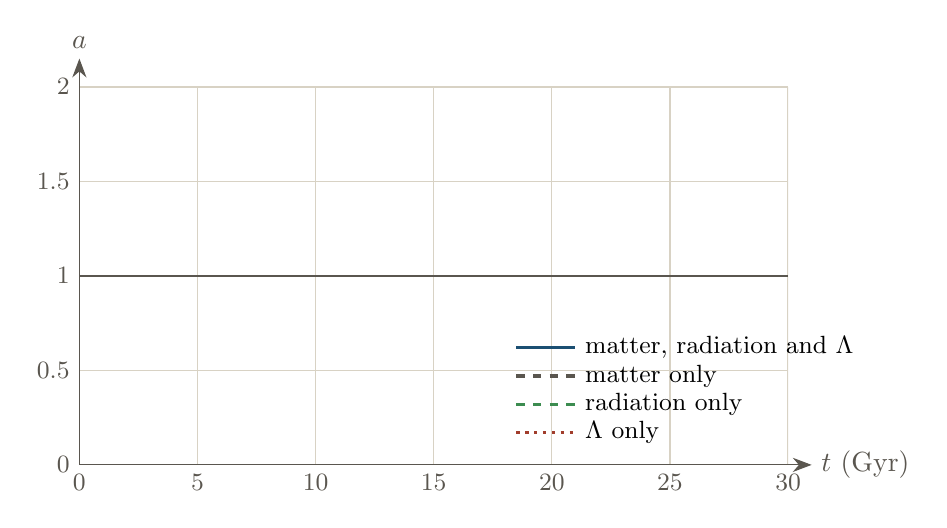
\begin{tikzpicture}[x=0.3cm,y=2.4cm, >={Stealth[length=2.4mm]}]
  \begin{scope}
    \clip (0,0) rectangle (30,2);
    \draw[linecol] (0,0) grid[xstep=5,ystep=0.5] (30,2);
    \draw[muted, dashed, line width=1.0pt] plot file {\datadir a_of_t_matter.dat};
    \draw[colthree, dashed, line width=1.0pt] plot file {\datadir a_of_t_radiation.dat};
    \draw[accent, dotted, line width=1.2pt] plot file {\datadir a_of_t_lambda.dat};
    \draw[astroblue, line width=1.4pt] plot file {\datadir a_of_t_lcdm.dat};
  \end{scope}
  \draw[->, muted] (0,0) -- (31,0) node[right] {$t\ (\mathrm{Gyr})$};
  \draw[->, muted] (0,0) -- (0,2.15) node[above] {$a$};
  \foreach \x in {0,5,10,15,20,25,30} \node[below, muted] at (\x,0) {\small \x};
  \foreach \y in {0,0.5,1,1.5,2} \node[left, muted] at (0,\y) {\small \y};
  \draw[muted, line width=0.6pt] (0,1) -- (30,1);
  \foreach \c/\st/\lab/\y in {astroblue/solid/{matter, radiation and $\Lambda$}/0.62, muted/dashed/{matter only}/0.47, colthree/dashed/{radiation only}/0.32, accent/dotted/{$\Lambda$ only}/0.17} {
    \draw[\c, line width=1.2pt, \st] (18.5,\y) -- (21,\y); \node[right] at (21,\y) {\small \lab};
  }
\end{tikzpicture}
\end{document}
